% Template for ICME 2018 paper; to be used with:
%          spconf.sty  - ICASSP/ICIP/ICME LaTeX style file, and
%          IEEEbib.bst - IEEE bibliography style file.
% --------------------------------------------------------------------------
\documentclass{article}
\usepackage{spconf,amsmath,epsfig}

\pagestyle{empty}


\begin{document}\sloppy

% Example definitions.
% --------------------
\def\x{{\mathbf x}}
\def\L{{\cal L}}


% Title.
% ------
\title{A Hybrid System Integrating Calibration and Registration for Accurate 3D Reconstruction}
%
% Single address.
% ---------------
\name{Anonymous ICME submission}
\address{}


\maketitle


%
\begin{abstract}
With the development of virtual and augmented reality, indoor 3D reconstruction based on multi-camera system has become increasingly popular recently. The quality of the reconstruction relies on many factors, including the multi-view camera parameters and the depth estimation in single view. To improve the final 3D model, we propose a new method to optimize and adjust the camera extrinsic parameters of the multi-camera system for high-quality 3D reconstruction. Our method consists of two parts: the global multi-camera calibration and the parameters refinement by point cloud registration. In global multi-camera calibration, we use checkerboard corners to optimize the camera extrinsic parameters globally obtained by pairwise camera calibration methods. In parameters refinement, we use ICP (Iterative Closest Point) to register the point clouds in different views reconstructed from the RGB and depth images. Then we use the transformation from ICP to adjust the extrinsic parameters to minimize the error caused by the depth estimation. The experimental results show our reconstructed results are precise and the effect of adjustment is promising.
\end{abstract}
%
\begin{keywords}
Multi-camera System, 3D reconstruction, camera calibration, four, five
\end{keywords}
%
\section{Introduction}
\label{sec:intro}
Real-time indoor 3D reconstructions from multiple views have become more and more prevalent recent years~\cite{dou2016fusion4d,orts2016holoportation}. Multi-camera systems using RGBD cameras have many advantages such as a wider horizon compared with the systems based on single camera, and are widely used in many kinds of applications. However, both the intrinsic and extrinsic parameters of the multi-camera systems are required to be calibrated accurately in order to achieve a high-quality and real-time 3D reconstruction of an entire object like people or furniture with less error.

For a single camera system, the accurate intrinsic parameters can be achieved by many internal calibration methods or toolboxes~\cite{zhang2000flexible,zhang2004camera}. Many efficient methods have also been developed for the calibration of different types of multi-camera calibration. One widely proposed approach for the multi-camera calibration is to use special calibration objects, such as  patterns, rig or similar. Li~\cite{Li2013A} proposed a toolbox to calibrate the system which uses a feature descriptor based calibration pattern. The pattern can be automatically detected even if the pattern is partially seen in an image. The toolbox yields good results especially on the systems with few cameras (three or four) with minimal overlapping fields of view. Zhao~\cite{zhao2008practical} proposed an algorithm based on 1D objects which works well on a triple camera system. The algorithm integrates the rank-4 factorization with the standard 1D camera calibration method and is much more convenient than the plane-based algorithm. Svoboda~\cite{svoboda2005convenient} gives a method only required any bright-spot object like a laser pointer. Waving the object which can be easily detected in each image through the working space is the only work requested. Kalibr~\cite{Maye2013Self} is a free toolbox that solves the multiple camera calibration problems. It can get a good estimate but requires that neighbouring cameras have overlapping fields of view. However, if the system contains many cameras and they do not share the same overlapping fields of view, the calibration process should be simply repeated for each pair of cameras.

Another kind of methods which is commonly used is self-calibration. These methods do the calibration using the constraints and correspondences from the images without any special calibration objects. Bundler~\cite{snavely2006photo} is a structure-from-motion toolbox using the unordered images captured from different views. The pose of all cameras can be estimated by the 3D reconstruction. It uses SIFT keypoint detector~\cite{lowe2004distinctive} which works well on the outdoor scenery but weak on indoor cases because of the lack of the features. Vasconcelos~\cite{vasconcelos2012minimal} proposed a solution to calibrate a camera with two other calibrated cameras using independent pairwise point correspondences. Bushnevskiy~\cite{bushnevskiy2016multicamera} present a novel approach for the estimation of the geometry of the multi-camera system. The algorithm enforce constraints arising from the visible epipoles and is especially suitable for dome-like indoor cases.

All these methods use RGB images to calibrate the multi-camera system and achieve good results. However, 3D reconstruction system also use other kinds of sensors, like Near Infra-Red cameras (NIR). If there are such cameras within the system used to estimate the depth, the error of the final result of the 3D reconstruction not only comes from the calibration of the RGB cameras but also from the depth estimation. How to minimize the error of the whole reconstruction to achieve an accurate model is a problem.

In this paper, we present an efficient algorithm to optimize the extrinsic camera parameters for indoor 3D reconstruction. To avoid from accumulative error caused by the repetitive calibration for each pair of cameras, we use a global camera calibration method and optimize all the camera parameters consistently. Furthermore, we use the point cloud registration method to adjust the result of the calibration. This can effectively decrease the error result from the depth estimation and obtain a high-quality 3D reconstruction.



\section{Overview}
Our algorithm consists of two main parts. Firstly, we use the toolbox Kalibr~\cite{Maye2013Self} to calibrate our multi-camera system and achieve the intrinsic and initial extrinsic parameters of all our cameras. Then we use a checkerboard as the calibration object, detect the corners on it and do the global extrinsic parameters optimization, as described in Sec. 3.3. Secondly, we use the camera parameters and the input rgb and depth images to reconstruct the point clouds of the model and use ICP (Iterative Closest Point)~\cite{Besl1992A} to align the point clouds of different views. Then the extrinsic parameters can be refined by the ICP transform to minimize the error caused by depth estimation, as described in Sec. 4. We compute the reprojection error and use a plaster model as ground truth to verify the effectivity of our algorithm, as described in Sec. 5.


\section{Global Camera Calibration}
The cameras in our 3D reconstruction system are placed on the periphery of the room pointing inwards, only the neighbouring cameras have overlapping fields of view. We found that if we calibrate the cameras pairwisely, accumulative error will occur and can be seen obviously in the result of the reconstruction. After the initial calibration, we optimize the extrinsic parameters globally using a checkerboard.

\subsection{Multi-camera System}

We employ 8 camera pods around the working space looking inwards for a full capture as shown in Figure~\ref{fig:rig}. Each pod consists of a color camera and 2 Near Infra-Red cameras (NIR). a laser pointer is used to produce special patterns, with it depth images can be achieved by the 2 NIR cameras using depth estimation methods.

\begin{figure}[h]
\centering
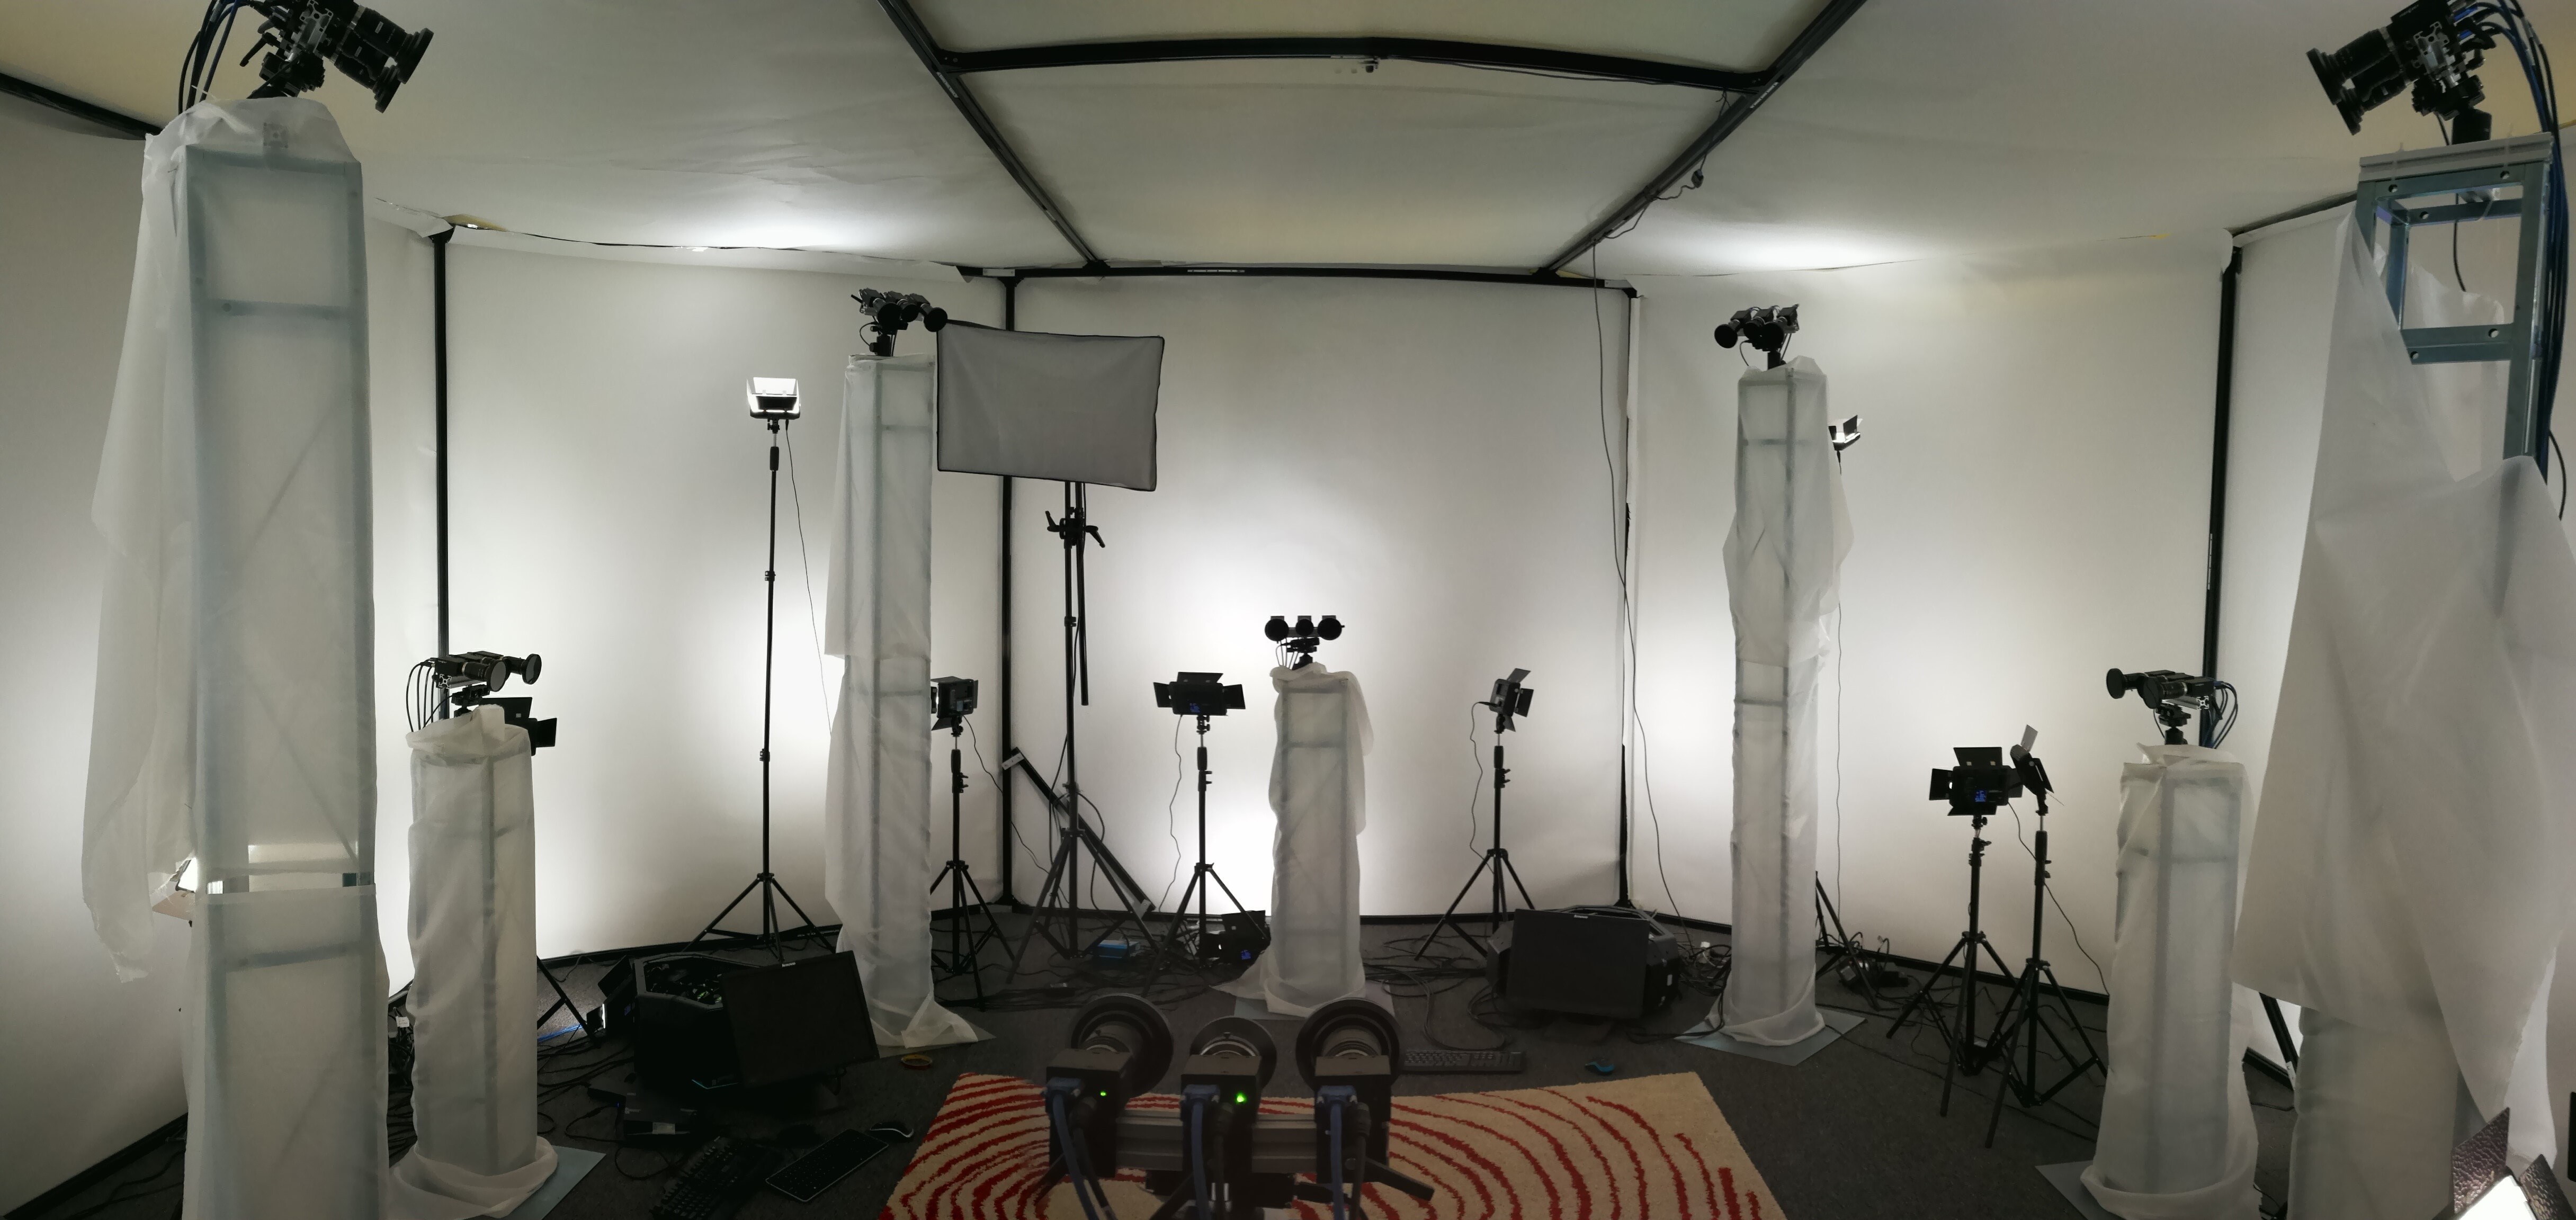
\includegraphics[scale=0.066]{rig.jpg}
\caption{Our multi-camera system with 8 camera pods pointing inwards.}
\label{fig:rig}
\end{figure}
\subsection{Camera Model}
Let $\mathbf{P}$ be the 3D space coordinates of a point $\emph{P}$, and $\mathbf{p}$ the 2D coordinates of its projection in the image plane, the model of a pin-hole camera is usually described as
\begin{equation}
z_{p}\mathbf{p}=\mathbf{K_{in}}\mathbf{K_{ex}}\mathbf{P},
\end{equation}
where $z_{p}$ is the projective depth of point $\emph{P}$, $\mathbf{K_{in}}$ and $\mathbf{K_{ex}}$ are the intrinsic and extrinsic parameters of the camera.
\subsection{Initial Calibration}
The $\mathbf{K_{in}}$ and initial $\mathbf{K_{ex}}$ of each camera are calibrated by Kalibr~\cite{Maye2013Self} pairwisely because of the lack of the common overlapping fields of view, including the 8 color cameras' extrinsic parameters $\{\mathbf{K_{ex}}_{i}\}_{i=1,...,8}$. The extrinsic parameters from the 2 NIR cameras to the color camera in the same camera pod are also achieved, but these extrinsic parameters are fixed and used to estimate the depth in each view.

\subsection{Global Optimization}

We use a $6\times7$ checkerboard with squares of 117 mm for the optimization. The user is requested to move the checkerboard in front of the cameras freely in the working space. The checkerboard can be simultaneously seen in three or four views usually. Then the 42 corners on the checkerboard can be detected in each group. We can estimate the 3D space coordinates $\mathbf{P_{c}}$ of each corner from the corresponding 2D coordinates $\{\mathbf{p_{c}}_{j}\}_{j=1,...,n}$, where $n$ is the number of the views that the checkerboard can be seen in at the same time. To make the optimization result be more consistent to the whole system, we also use the images with checkerboard on the ground which allows the checkerboard corners can be seen in all the 8 cameras. This will help to reduce the accumulative error and inconsistence caused by the pairwise calibration. The aim of the optimization is to minimize the sum of all reprojection errors with respect to all 3D point and extrinsic parameters, which is described as
\begin{equation}
E(\{\mathbf{K_{ex}}_{i}\})=\sum_{i}\sum_{j}((\mathbf{K_{in}}_{i}\mathbf{K_{ex}}_{i}\mathbf{P_{c}}_{j})-\mathbf{p_{c}}_{ij})^{2}.
\end{equation}

We use an open source software package called sba to solve this problem~\cite{lour09}.


\begin{figure}[ht]
%
\begin{minipage}[b]{.48\linewidth}
  \centering
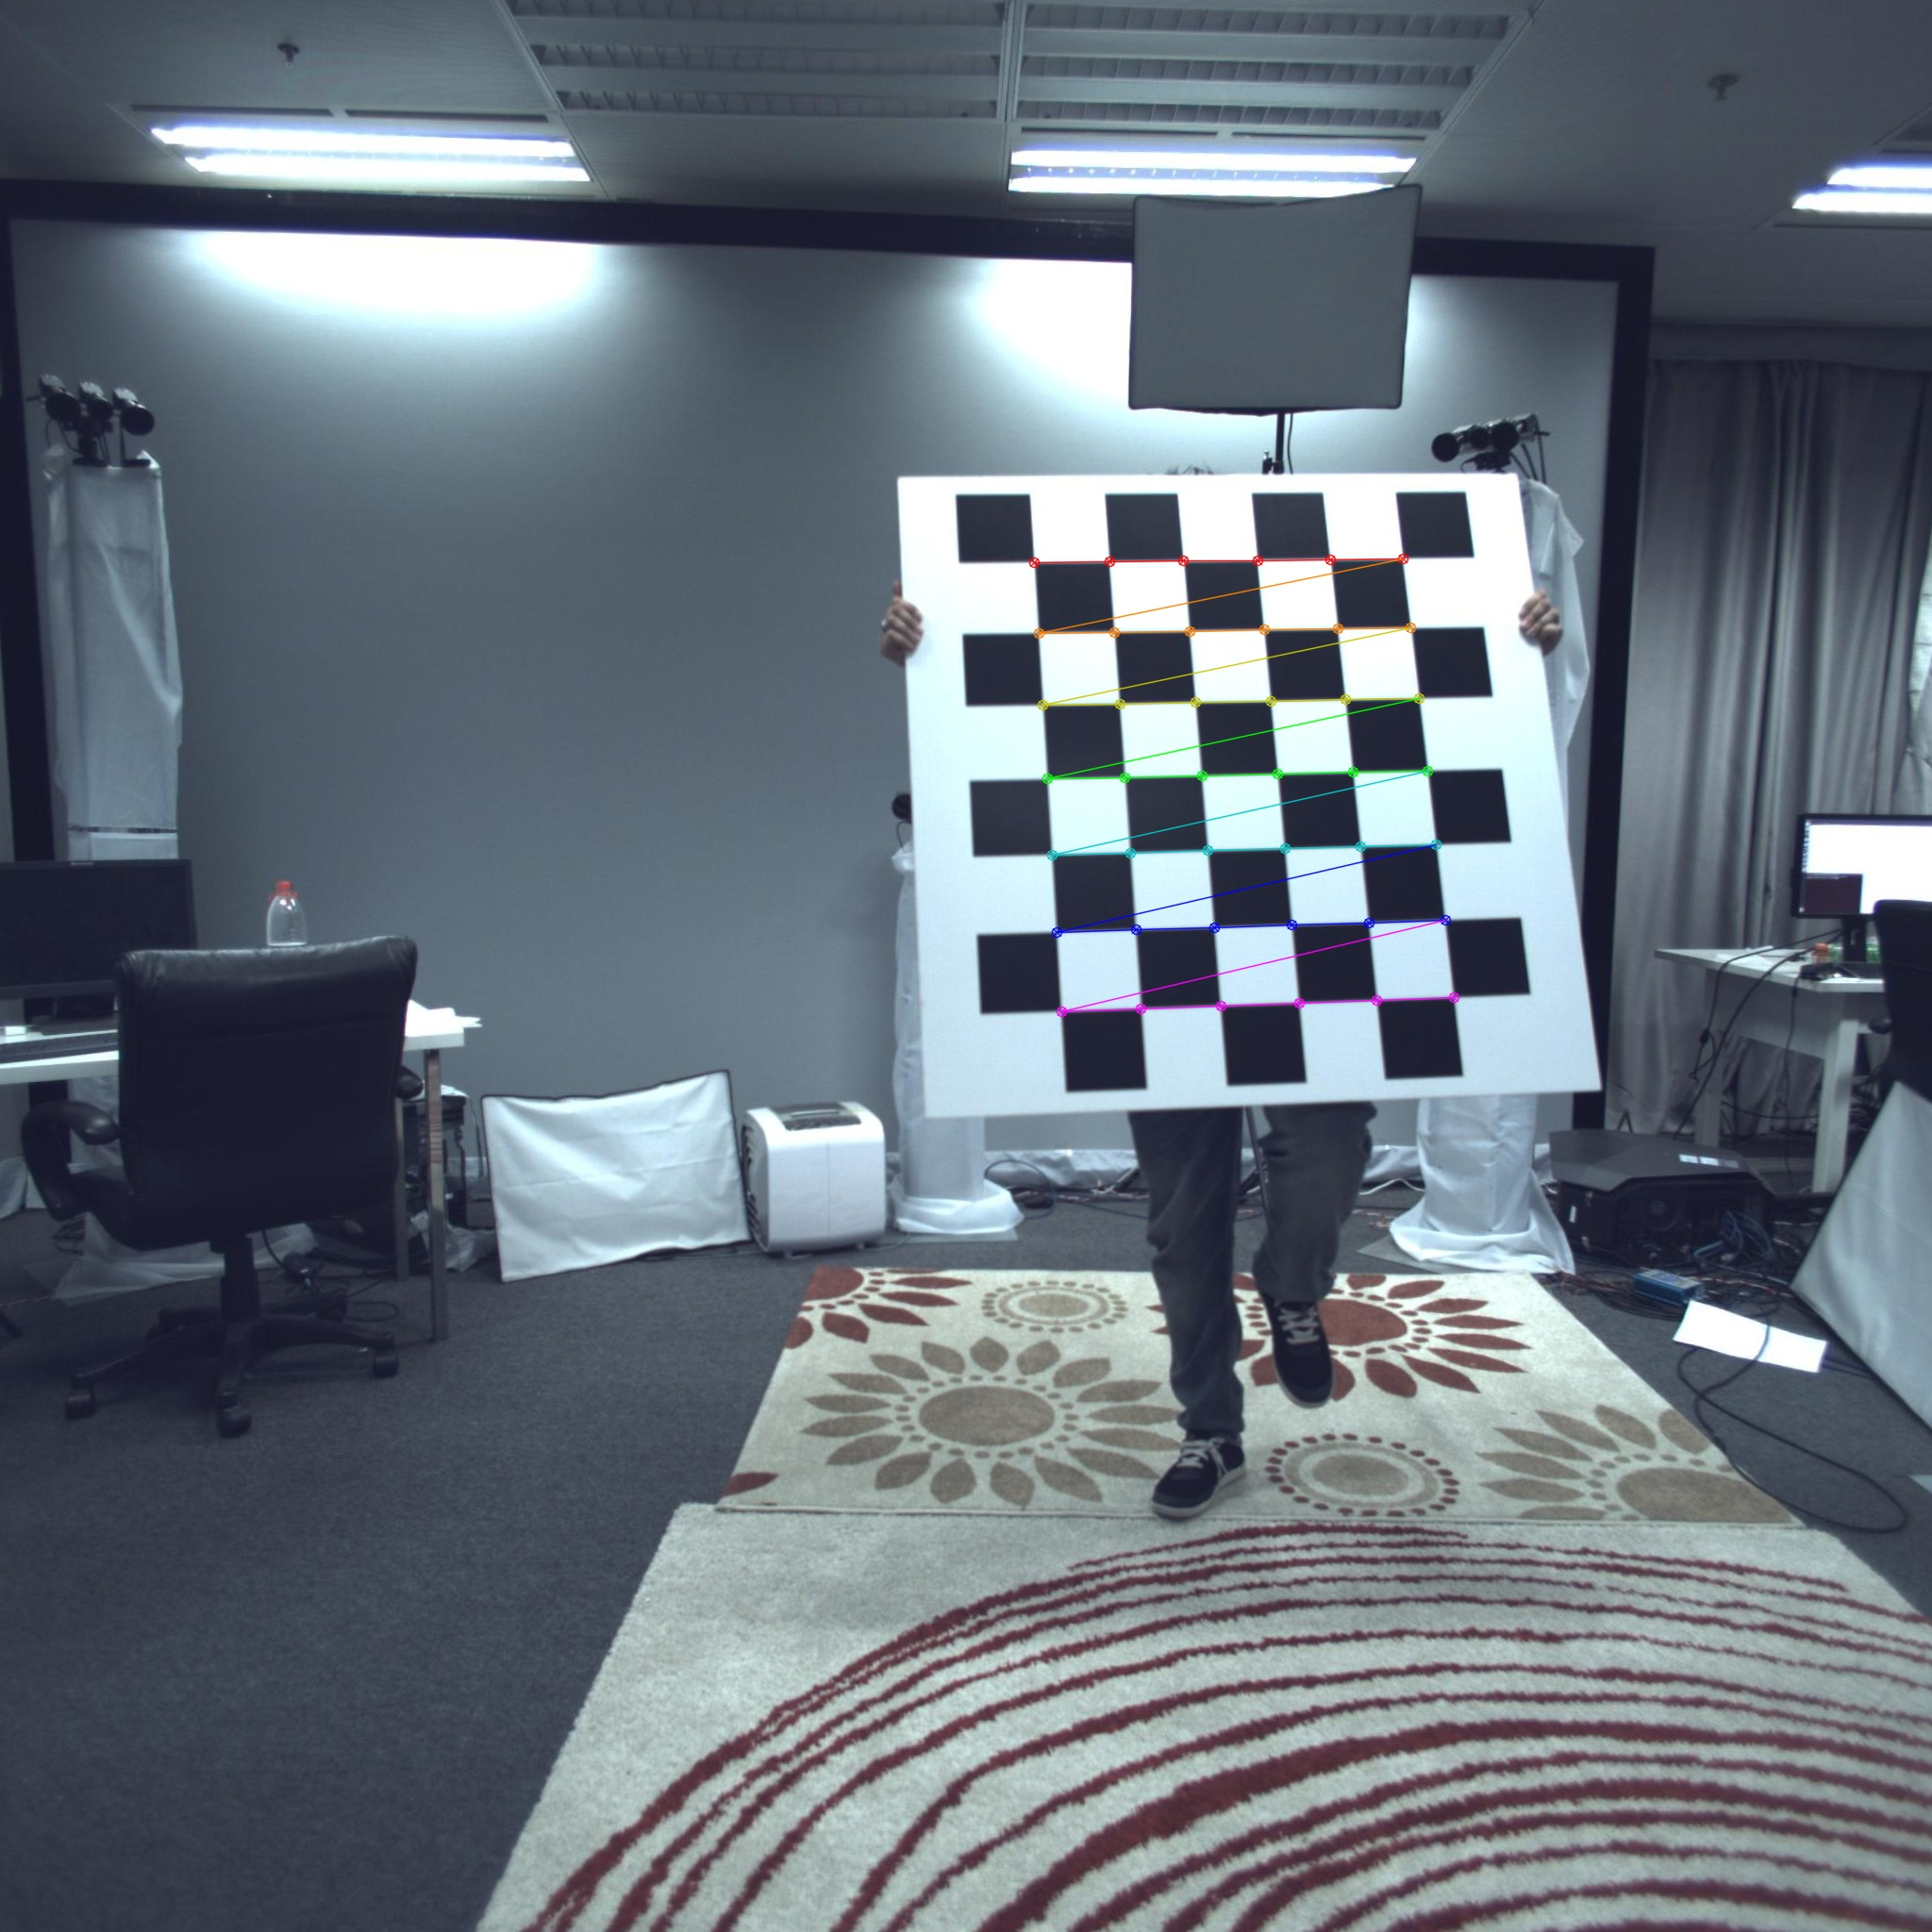
\includegraphics[scale=0.058]{free.jpg}
  \vspace{0cm}
  \centerline{(a)}\medskip
\end{minipage}
\hfill
\begin{minipage}[b]{0.48\linewidth}
  \centering
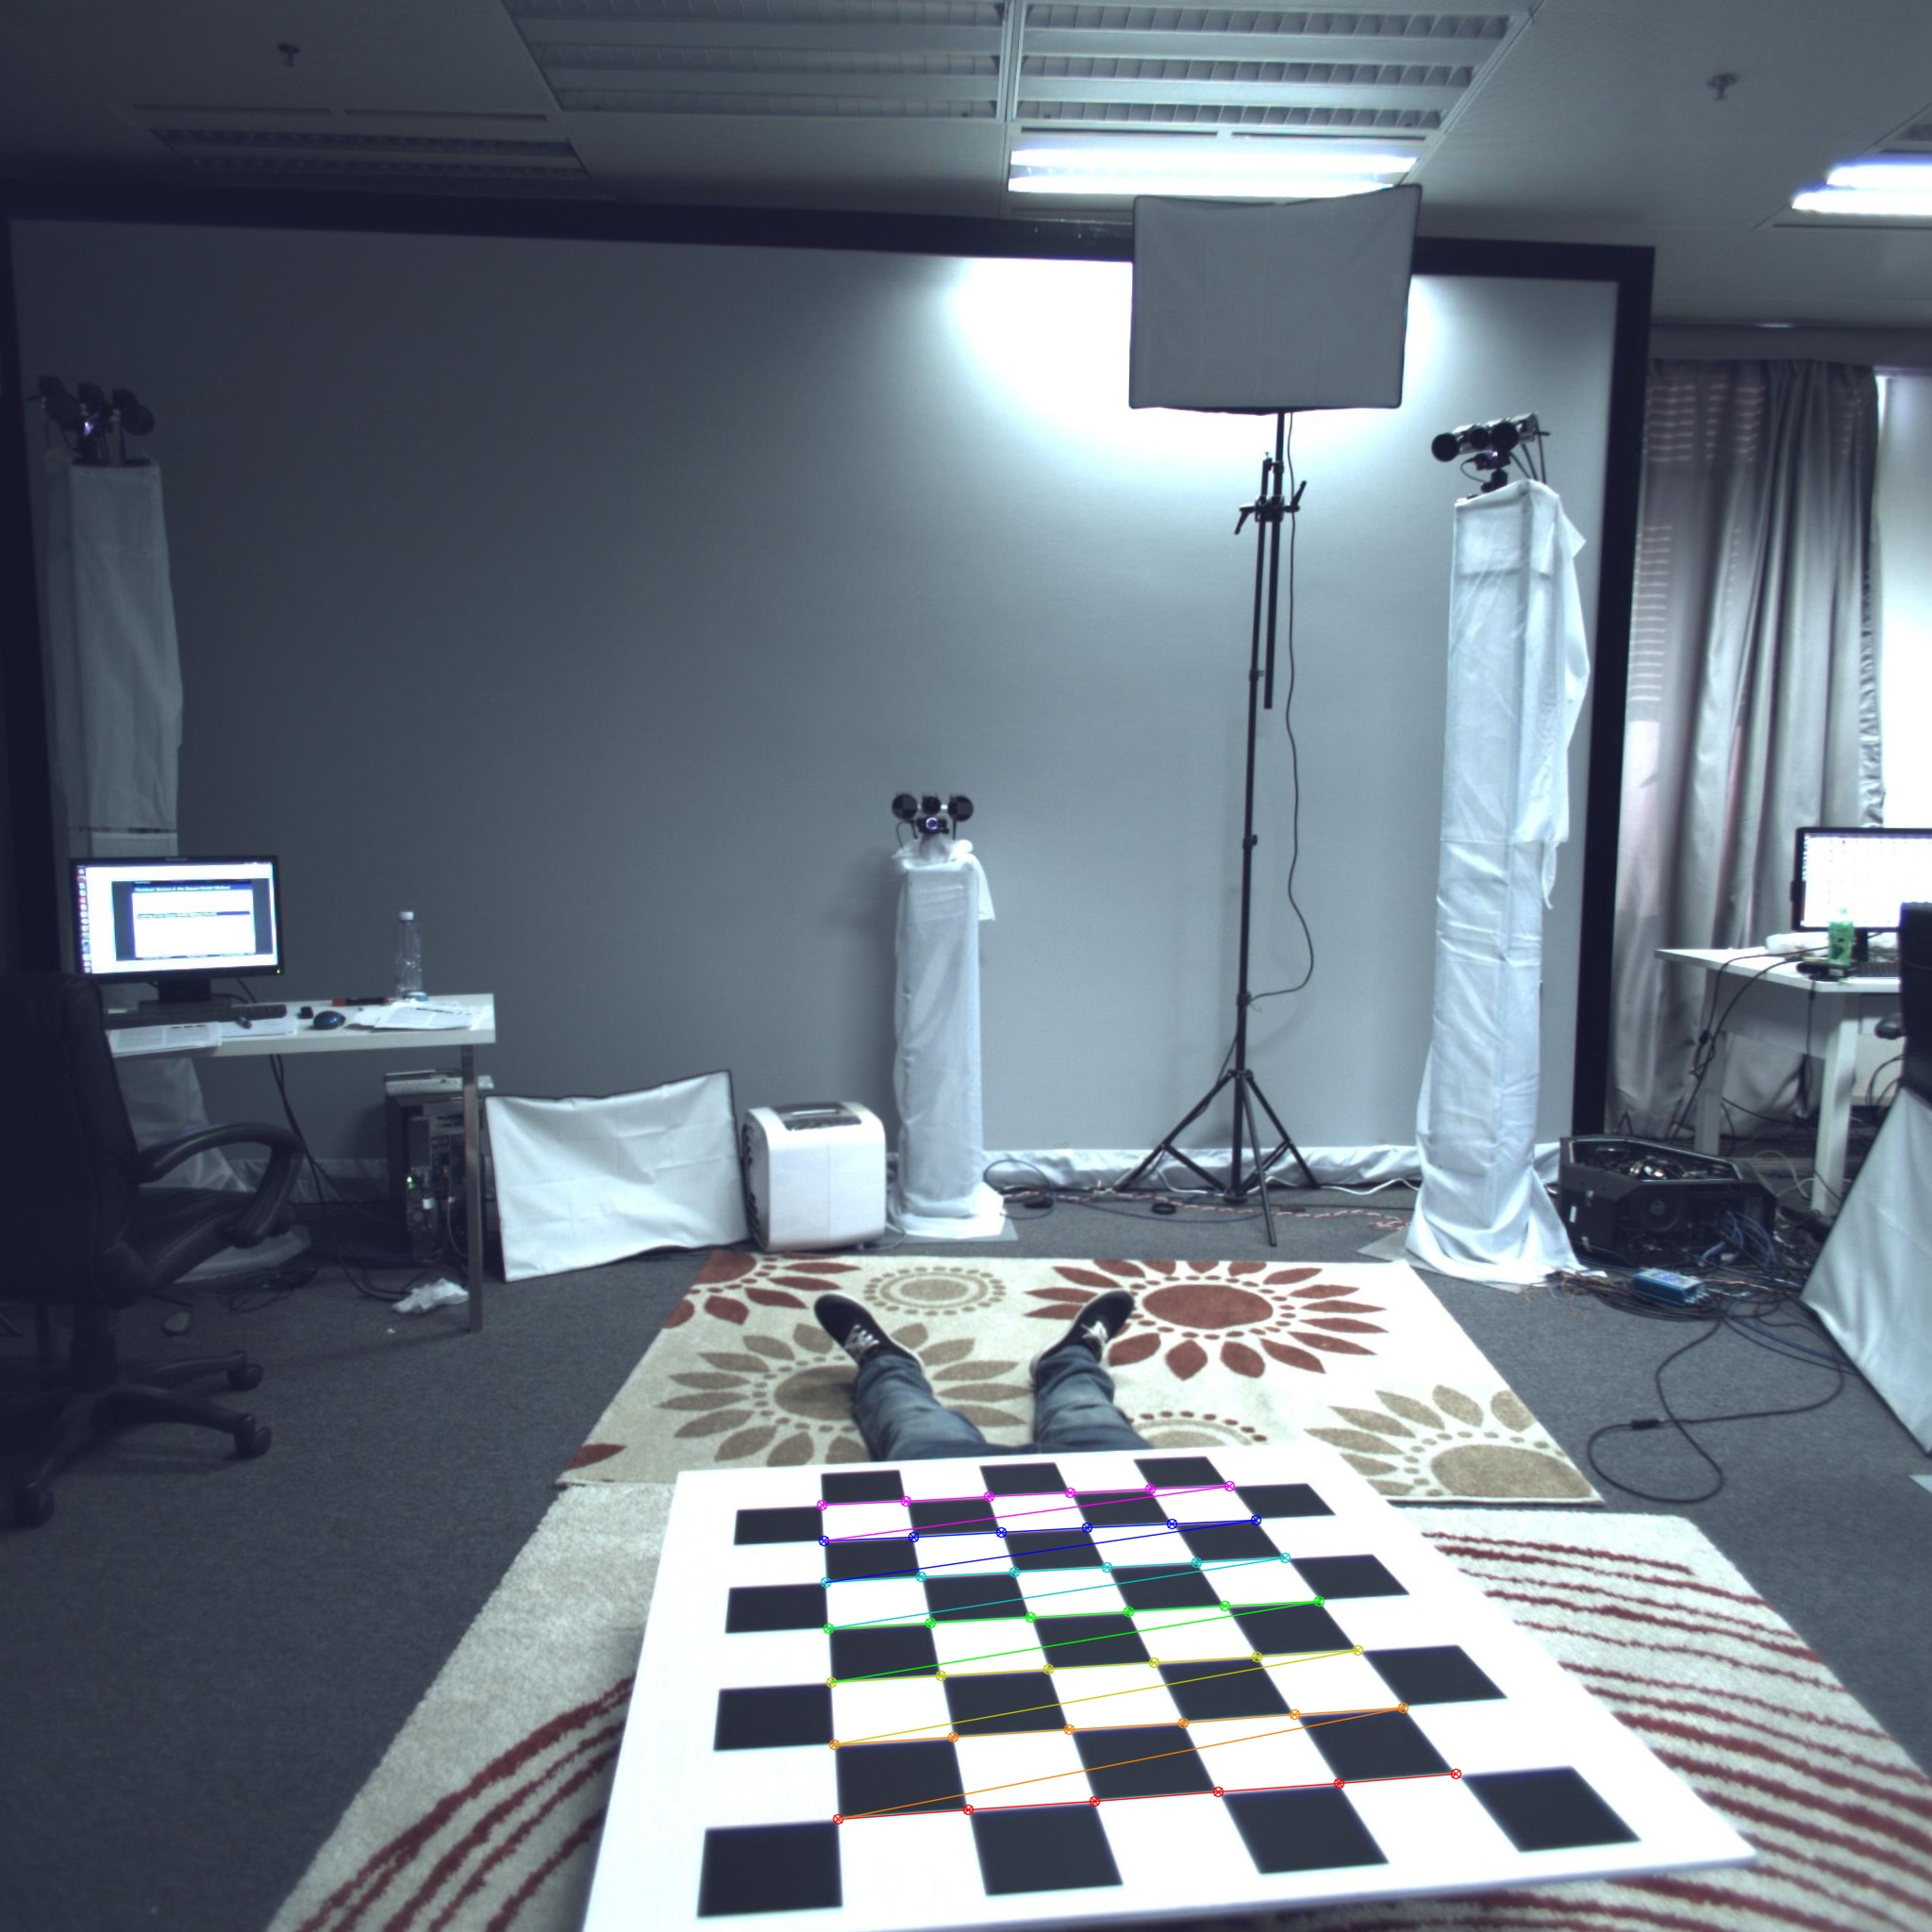
\includegraphics[scale=0.058]{ground.jpg}
  \vspace{0cm}
  \centerline{(b)}\medskip
\end{minipage}
%
\caption{Results of the checkerboard corners detection. (a): Results when the user moves freely. (b): Results when the checkerboard is on the ground. }
\label{fig:res}
\end{figure}
\section{refinement by point cloud registration}

We achieve the depth data from the 2 NIR cameras using depth estimation methods. Although after the global optimization, we can get a result with less reprojection error, but it may not be the optimal solution to the 3D reconstruction beacause the quality of depth estimation also influence the final result. If the depth and camera parameters are both accurate enough, the point clouds of different views should align very well. However, the error cannot be avoided completely. To minimize the error from depth data and get a high-quality reconsturction, We use ICP to refine the extrinsic parameters by point cloud registration.

For each point reconstructed by the depth image, we consider an estimation
\begin{equation}
\mathbf{\tilde{P}}_{ij}=f_{i}(\mathbf{P}_{j}),
\end{equation}
where $\mathbf{P}_{j}$ is the true 3D coordinates in the camera coordinate system. $f_{i}$ is a nonlinear function for view $i$, represent the depth influence. $\mathbf{\tilde{P}}_{ij}$ is the 3D coordinates we get from the depth data and intrinsic parameters in view $i$. With the extrinsic parameter, we can transform all the points into the world coordinate system. The estimation can be written as
\begin{equation}
\mathbf{\hat{P}}_{gj}=g(\mathbf{K_{ex}}_{i})f_{i}(\mathbf{P}_{j}),
\end{equation}
where $\mathbf{\hat{P}}_{gj}$ is the 3D coordinates in the world coordinate system we reconstruct from the depth and camera parameters. ICP can be replaced as a rigid transform to all views
\begin{equation}
\mathbf{\tilde{\hat{P}}}_{gj}=M_{i}g(\mathbf{K_{ex}}_{i})f_{i}(\mathbf{P}_{j})=g(\mathbf{K_{ex}}_{i})M_{i}f_{i}(\mathbf{P}_{j}),
\end{equation}
where $\mathbf{\tilde{\hat{P}}}_{gj}$ is the coordinates of the point after the alignment. The transform $M_{i}$ can refine the error caused by $f_{i}$, and improve the quality of the result of 3D reconstruction.

We choose the point cloud of view 1 as the reference, align the point cloud of view 2 to it, combine the result of the two views, then align the point cloud of view 3 to the combined result and so on. Each ICP process produce a transformation matrix, then we can refine the extrinsic parameters using the rigid transformation.
\section{EXPERMENTS}

\subsection{reprojection error}

\subsection{plaster model}

\section{conclusion}


% References should be produced using the bibtex program from suitable
% BiBTeX files (here: strings, refs, manuals). The IEEEbib.bst bibliography
% style file from IEEE produces unsorted bibliography list.
% -------------------------------------------------------------------------
\bibliographystyle{IEEEbib}
\bibliography{icme2018template}

\end{document}
